
\chapter{Results}


XXX - CV needs pictures. 
look at 5.5.,m visualize maybe
single image for match not side by side. - not clear what its finding, but it is robust which is nice - try ask what are these dots... what are keypoints 
- GitHub link for code. Mentionthis is how it was implemented, not flow diagram. So when someone goes on Github they know whats going on.
Crop Earth 
overlap relative to my baseline image 972. no 1080.  

\section{Detailed Performance Analysis}

This section presents the results achieved by the navigation system under optimal conditions across various challenging datasets. The analysis focuses on the system's performance in terms of accuracy, efficiency, and generalizability, providing insights into its applicability in real-world UAV navigation scenarios.

xxx - show matches black and white. 
make a note linking setup for testing phase xxx
\subsection{Key Performance Metrics}


The system's generalized performance across five diverse datasets—CITY1, CITY2, ROCKY, DESERT, and AMAZON— is summarized by its Accuracy and Runtime. 

Accuracy is measured in two broad potential ways. 

The first is the the absolute radial error, or RMSE, in GPS coordinates, either for the mean of the dataset or per image, in metres. This provides a physical understanding of the error scope and a nuanced understanding of the inelasticity of the system to the movement size. This may also be represented in pixels, or axial components; the former provides an intuition behind the error size given a fixed resolution of 1920x972 pixels

Secondly is the relative radial error which is measured as a percentage of the actual radial distance, in equivalent metrics. Specifically, the radial error is the radial error between the estimated and actual GPS coordinates, in metres, while the radial distance is the magnitude of the translation vector from the centre of the reference image to that of the current image, in metres. This provides a normalized measure of the error relative to the movement size, allowing for a more intuitive understanding of the system's accuracy. This may also be represented axial component.



say what the times are. say acc and time 



% Table 2: Absolute Radial Error in Metres
\begin{table}[H]
    \centering
    \caption{\textbf{Percentage Radial Error (Relative Deviation)}}
    \label{tab:percentage_radial_error}
    \begin{tabular}{|l|c|c|c|c|c|}
    \hline
    & \textbf{CITY1} & \textbf{CITY2} & \textbf{ROCKY} & \textbf{DESERT} & \textbf{AMAZON} \\
    \hline
    \makecell{\textbf{Percentage} \\ \textbf{Radial Error (\%)}} & 0.37220028 & 0.2383268 & 0.71984452 & 0.24183624 & 0.38495021 \\
    \hline
    \end{tabular}
\end{table}


% Table 3: Radial Errors in Pixels
\begin{table}[H]
\centering
\caption{\textbf{Radial Errors in Pixels (Min, Mean, Max)}}
\label{tab:radial_errors_pixels}
\begin{tabular}{|l|c|c|c|c|c|}
\hline
& \textbf{CITY1} & \textbf{CITY2} & \textbf{ROCKY} & \textbf{DESERT} & \textbf{AMAZON} \\
\hline
\makecell{\textbf{Mean Pixel} \\ \textbf{Error}} & 0.7221 & 0.6120 & 1.0303 & 0.5677 & 0.3914 \\
\hline
\makecell{\textbf{Max Pixel} \\ \textbf{Error}} & 2.1735 & 1.0046 & 4.9199 & 1.7750 & 1.0556 \\
\hline
\end{tabular}
\end{table}


% Table: Radial Errors in Meters (Mean, Max)
\begin{table}[H]
    \centering
    \caption{\textbf{Radial Errors in Meters (Mean, Max)}}
    \label{tab:radial_errors_meters}
    \begin{tabular}{|l|c|c|c|c|c|}
    \hline
    & \textbf{CITY1} & \textbf{CITY2} & \textbf{ROCKY} & \textbf{DESERT} & \textbf{AMAZON} \\
    \hline
    \makecell{\textbf{Mean Meter} \\ \textbf{Error}} & 
        2.9390 & 
        1.9124 & 
        3.1922 & 
        1.7598 & 
        1.3412 \\
    \hline
    \makecell{\textbf{Max Meter} \\ \textbf{Error}} & 
        8.8451 & 
        3.1394 & 
        15.2403 & 
        5.5047 & 
        3.6141 \\
    \hline
    \end{tabular}
    \end{table}
    

% Table 4: Time Table
\begin{table}[H]
\centering
\caption{\textbf{Processing Times (Seconds)}}
\label{tab:processing_times}
\begin{tabular}{|l|c|c|c|c|c|}
\hline
& \textbf{CITY1} & \textbf{CITY2} & \textbf{ROCKY} & \textbf{DESERT} & \textbf{AMAZON} \\
\hline
\makecell{\textbf{Mean} \\ \textbf{Add Time}} & 0.7684 & 0.8343 & 0.6292 & 0.5347 & 0.6315 \\
\hline
\makecell{\textbf{Mean Parameter} \\ \textbf{Inference Time}} & 1.6257 & 1.7150 & 1.5806 & 1.7735 & 1.6855 \\
\hline
\makecell{\textbf{Mean Location} \\ \textbf{Inference Time}} & 1.6739 & 1.5714 & 1.5110 & 1.7827 & 1.4405 \\
\hline
\end{tabular}
\end{table}





. The results are presented in Figure \ref{fig:Key Metrics}. Importantly, the system meets the real-time requirement of 2 seconds and the accuracy requirement of 10\%. 

% the plot of key metrics with regard to system performance. 
\begin{figure}[H]
    \centering
    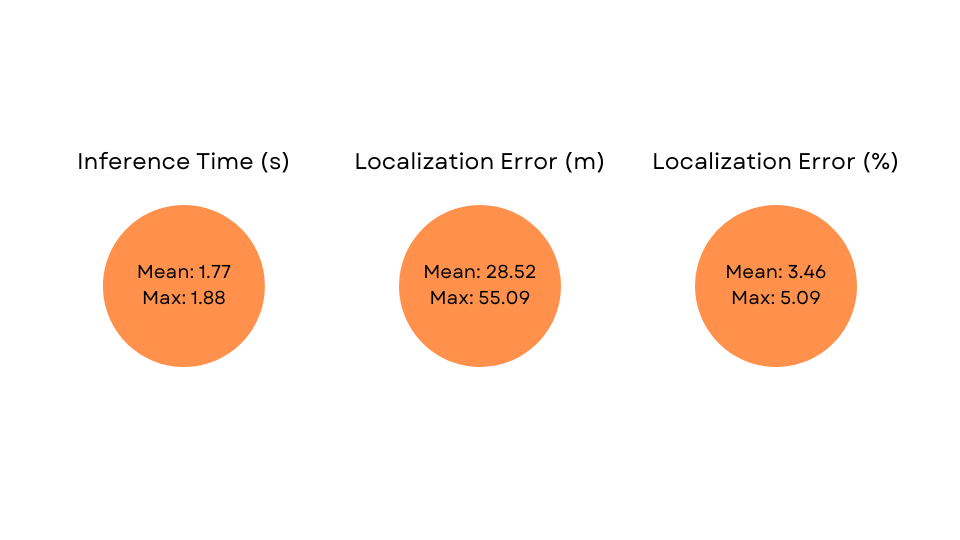
\includegraphics[width=0.8\textwidth]{./Chapter 5/RESULTPLOTS/Metrics_Raw.png}
    \caption{Key Accuracy And Runtime Performance Metrics}
    \label{fig:Key Metrics}
\end{figure}





\subsection{Flight Path Analysis}
Figures \ref{fig:Flight Path ROCKY} and \ref{fig:Flight Path DESERT} show the actual vs estimated flight of the UAV across the worst and best performing dataset, ROCKY and DESERT respectively. Even in the worst performing dataset, the system maintains a highly accurate flight path. On a global scale, this error is negligible. The pilot be able to control the UAV and prevent further drift under significantly worse conditions.


    \begin{figure}[H]
        \centering
        \begin{minipage}{0.45\textwidth}
            \centering
            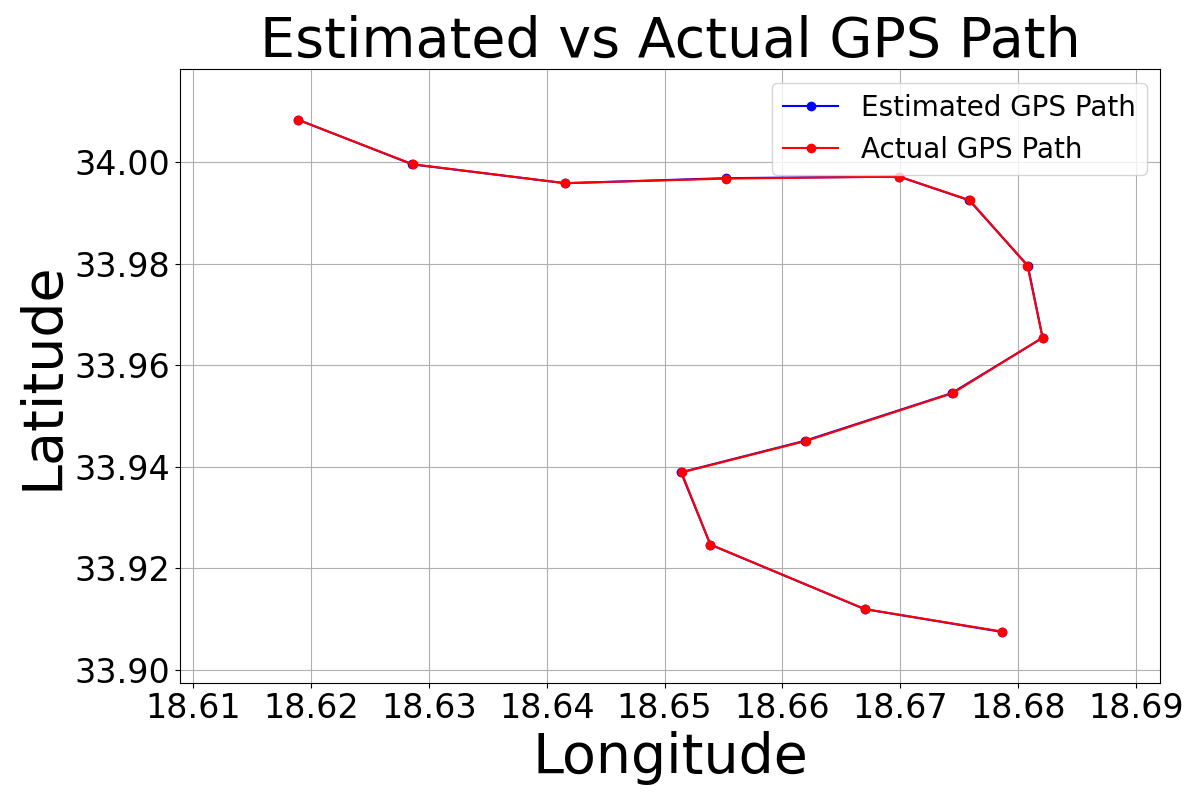
\includegraphics[width=0.7\textwidth]{./Chapter 5/GPSpaths/PathCity1.png}
            \caption{Flight Path of UAV in Rocky Dataset (Worst)}
            \label{fig:Flight Path ROCKY}
        \end{minipage}\hfill
        \begin{minipage}{0.45\textwidth}
            \centering
            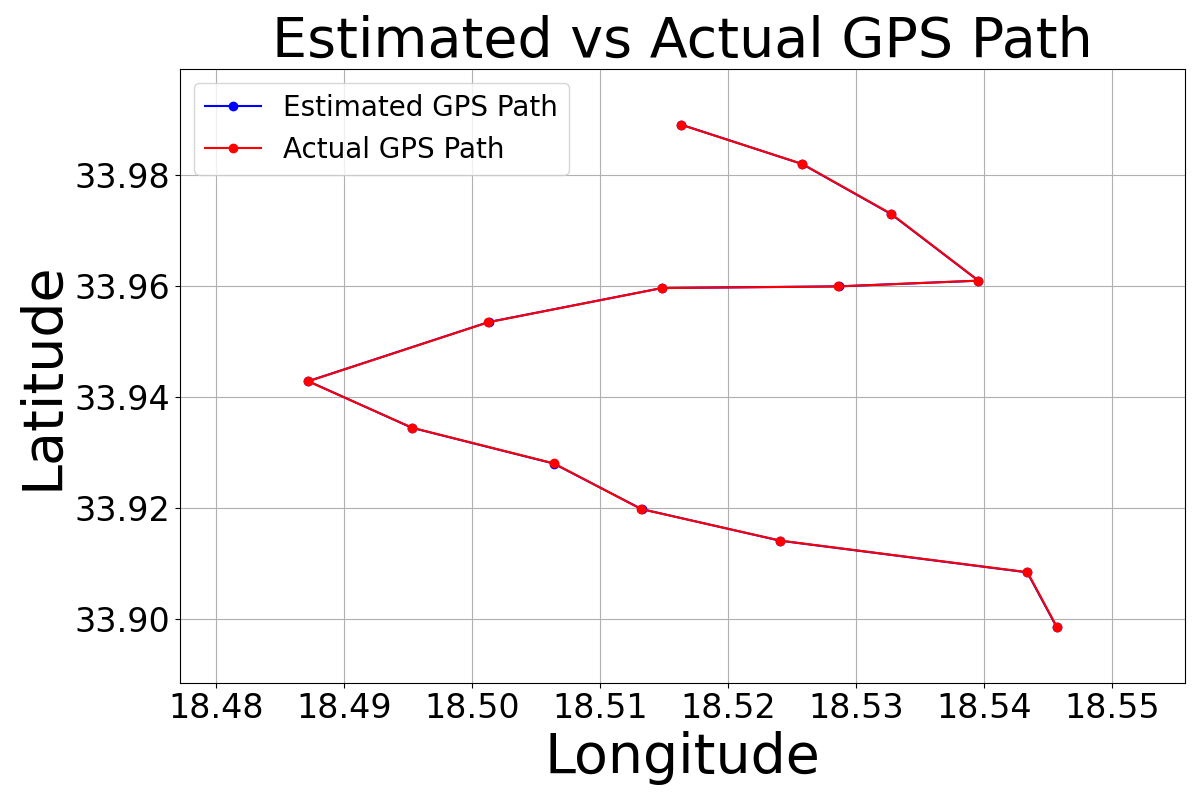
\includegraphics[width=0.7\textwidth]{./Chapter 5/GPSpaths/PathCity2.png}
            \caption{Flight Path of UAV in Desert Dataset (Best).}
            \label{fig:Flight Path DESERT}
        \end{minipage}
    \end{figure}


\subsection{Detailed Performance Metrics}
The detailed performance metrics include per dataset accuracy and time metrics. Namely, the radial RMSE error in GPS in meters and percentage, and the time taken for each stage of the pipeline, including the extraction and parameter inference time per while GPS is available, and the location inference time per image when GPS is lost. The results are summarized in Figures \ref{fig:Per Dataset Metrics} and \ref{fig:Per Dataset Metrics}. 

The results show that the system achieves consistent accuracy and runtime performance across each dataset. Further, its noted that both pipelines are able to maintain real-time performance, seen by the sum of the parameter inference and add times being below 2 seconds, as well as the location inference time being below 2 seconds. The accuracy of the system is also maintained, with the RMSE error being below 10\% for all datasets.


\begin{figure}[H]
    \centering
    \begin{minipage}{0.45\textwidth}
        \centering
        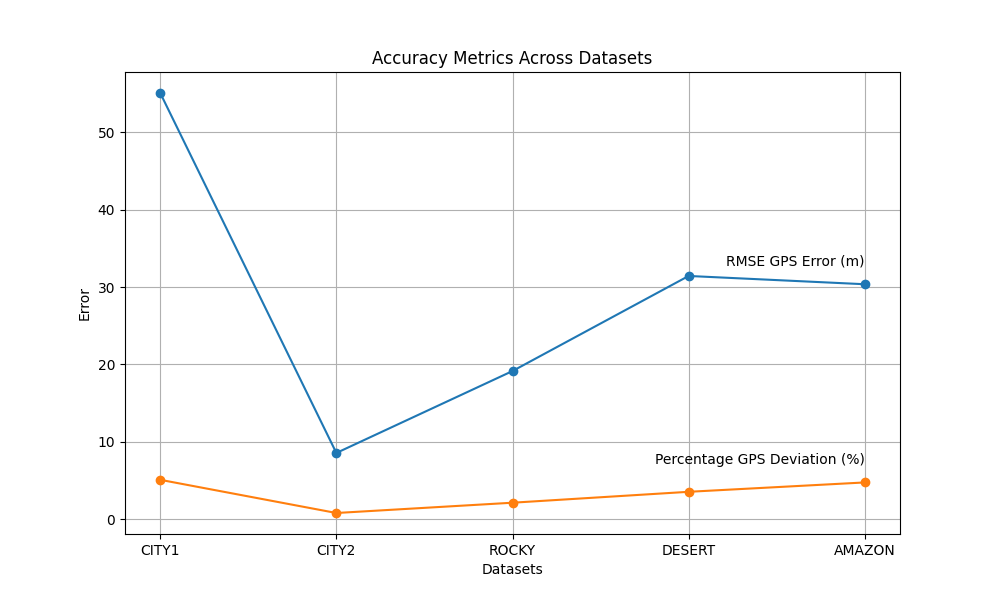
\includegraphics[width=\textwidth]{Chapter 5/RESULTPLOTS/key metrics/Accuracy Datasets.png}
        \caption{Accuracy Metrics for Each Dataset}
        \label{fig:Per Dataset Metrics}
    \end{minipage}\hfill
    \begin{minipage}{0.45\textwidth}
        \centering
        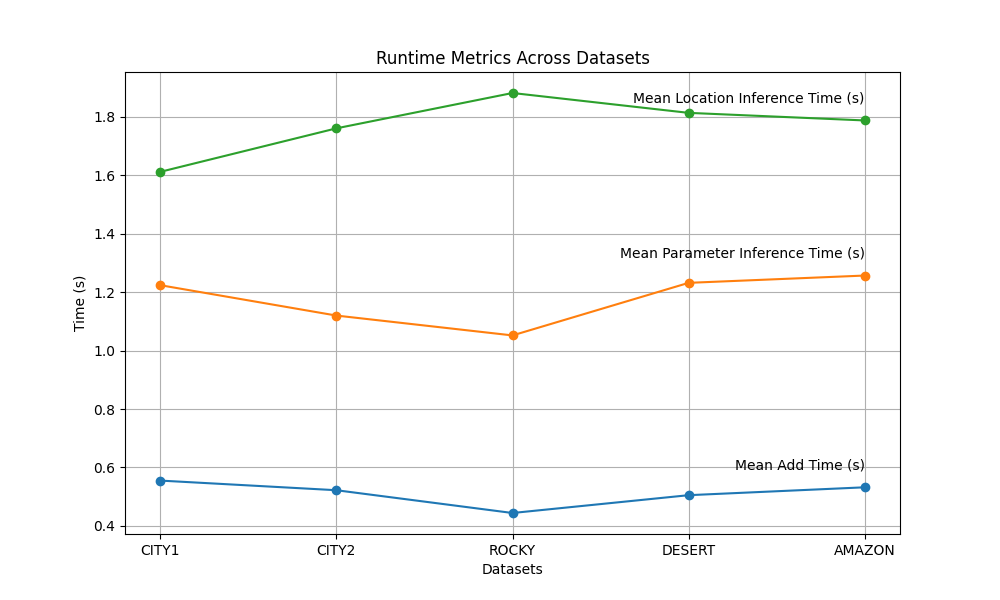
\includegraphics[width=\textwidth]{Chapter 5/RESULTPLOTS/key metrics/Runtime Datasets.png}
        \caption{Runtime Metrics for Each Stage of the Pipeline}
        \label{fig: Dataset Metrics}
    \end{minipage}
\end{figure}



\subsection{Dataset Performance Analysis}

This section utilizes the violin plot, in Figure \ref{fig:Violin Dataset Plot}, to visualize the statistical distribution of radial errors across each dataset. This plots details the mean, median, and variance of the radial errors, as well as the distribution of errors across the datasets. The results provide insights into the system's accuracy and robustness in diverse environments. 

The plot shows relatively consistent performance across datasets, with CITY2, being consistent with the global heading space, having the most accurate and reliable inter-dataset performance. The CITY1 and AMAZON datasets show comparitively high variation between their minimum and maximum errors, indicating a higher variance in direction.

\begin{figure}[H]
    \centering
    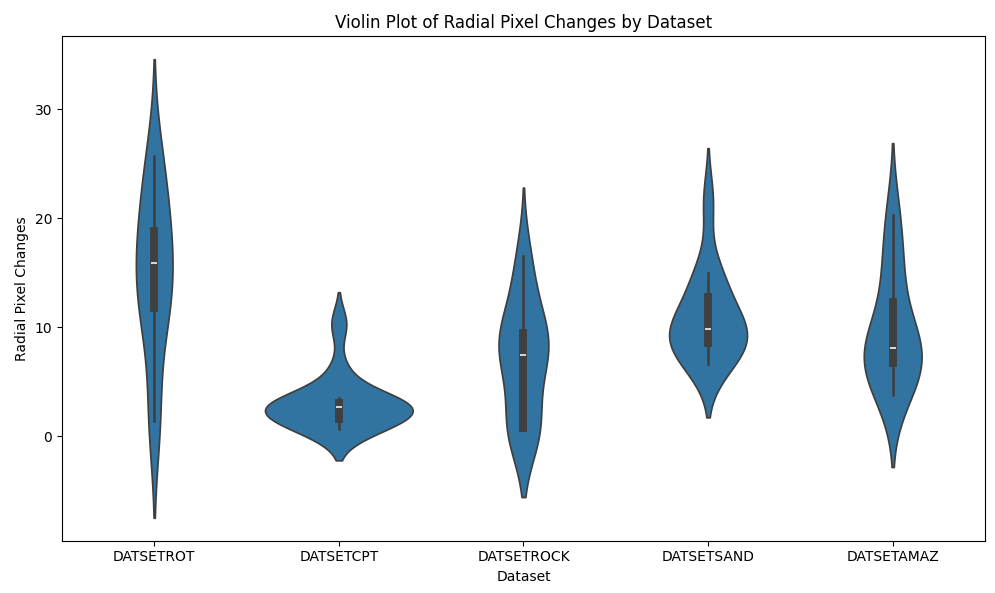
\includegraphics[width=0.7\textwidth]{Chapter 5/RESULTPLOTS/violindatasets.png}
    \caption{Plot of distribution of radial errors in each dataset}
    \label{fig:Violin Dataset Plot}
\end{figure}



\subsection{Error Distribution Map}

The heatmap in Figure \ref{fig:Heatmap_XY_Dev} illustrates the distribution of pixel deviations in the X and Y directions across the datasets. For spatial conciseness, some axial values are omitted, and the values are quantized into bins, meaning they are not exactly off by the pixel bin they are in. This visualization provides an intuitive understanding of the pixel error distribution and any potential axial bias. As shown, the errors are distributed relatively evenly across both axes, indicating no significant bias in the system. Moreover, the majority of errors are below 2 pixels, demonstrating the system's robustness and accuracy in localization estimates. The largest radial error, as noted in Table \ref{tab:radial_errors_pixels}, is 4.9199 pixels. While this error is relatively small, the sources of these errors are discussed in the following section.


\begin{figure}[H]
    \centering
    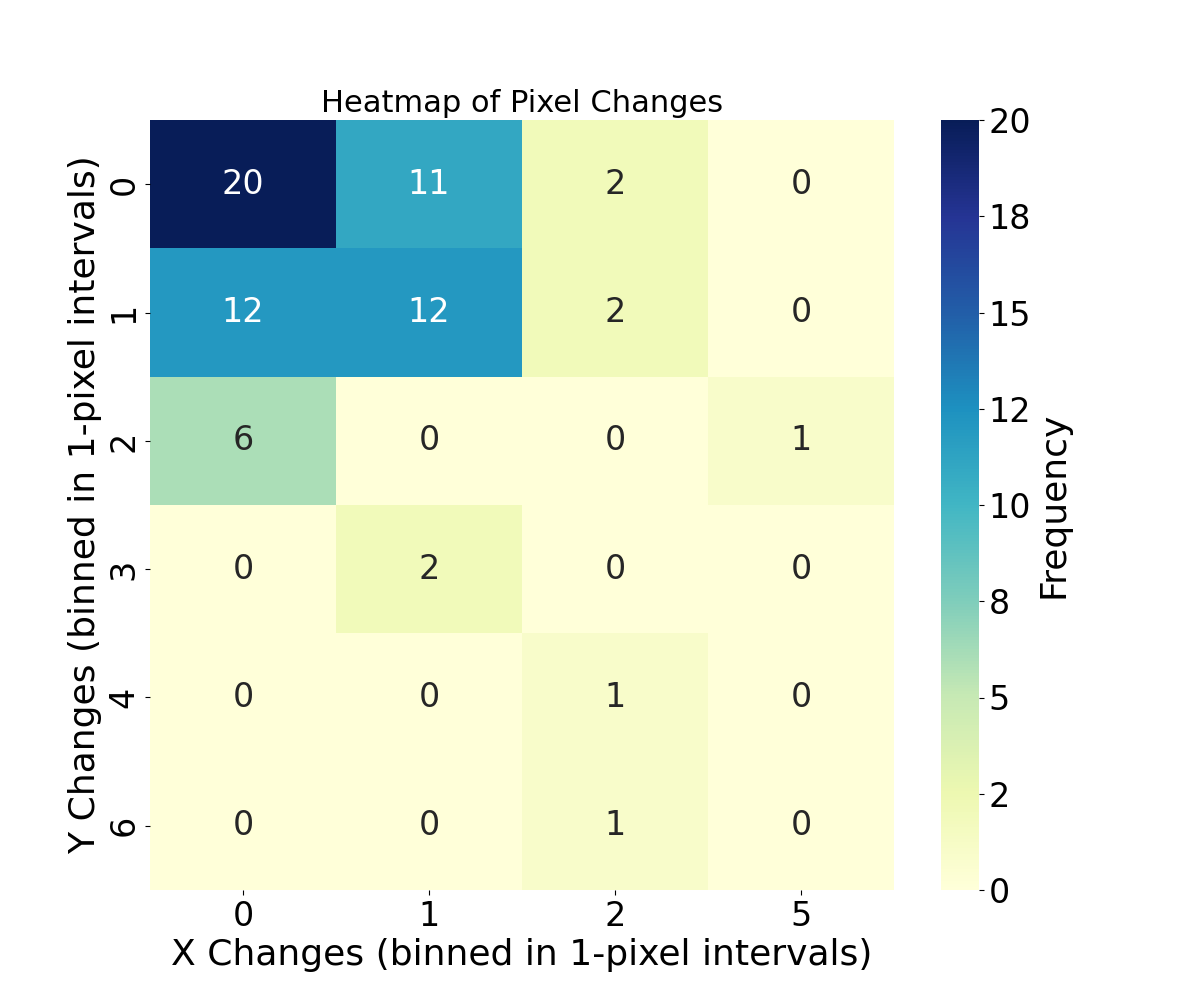
\includegraphics[width=0.65\textwidth]{Chapter 5/RESULTPLOTS/XYHEAT.png}
    \caption{Heatmap of Pixel Deviations in X and Y Directions}
    \label{fig:Heatmap_XY_Dev}
\end{figure}



\subsubsection{Sources of Error}

The performance of the UAV navigation system is influenced by several sources of error, which are detailed below:


\textbf{Quantization:} 
When images are taken from slightly different positions, feature edges can distort due to sub-pixel shifting. This is because a fixed resolution can averages any information smaller than a pixel. For large features, these distortions at feature boundaries are minimal relative to feature size, but for smaller features, edge distortions occupy a significant portion, leading to high levels of distortion. At high altitudes, where features are predominantly small, this effect distorts a large number of descriptors and keypoints, leading to considerable distortion.

This issue is prominent in the CITY datasets, where dense, small features amplify sub-pixel errors, leading to higher mean errors. While CITY2’s dataset also experiences sub-pixel shifting, it involves only significant translations rather than rotations, which has a larger impact on reducing distortion overall; hence, the error is not visible in the CITY2 dataset.

\textbf{Depth and Perspective Changes:} Google Earth uses a 3D model to generate its terrain, leading to changes in perspective and ground height as images are taken from different spots in the landscape. This effect is particularly evident in the ROCKY dataset, where large height changes in the mountainous regions cause both perspective distortion and scale changes.

\textbf{Variations in Terrain and Environmental Conditions:} Each terrain in the dataset has unique characteristics, including differences in feature count, contrast, and uniqueness. The optimal number of good features varies with the terrain. In this study, a static target number of keypoints was applied to each stage, which does not fully account for these differences. The system may generalize well across multiple datasets but it is not perfectly optimized for any specific one. A model that dynamically adjusts parameters or employs machine learning to optimize them would be more effective.

\textbf{Algorithmic Constraints:} The selected image processing and matching algorithms have inherent limitations, especially under extreme conditions or with highly repetitive features. Additionally, being optimized for efficiency, they may not capture and represent every feature within an image perfectly.

Despite these factors, the system's achieved radial error range of 0-5 pixels across datasets underscores its robustness and effectiveness, affirming its suitability for practical UAV applications.

\section{Stress Testing}

This section involves the analysis of the system's robustness under various stressful conditions, including low-light environments and reduced mutual information. These tests were chosen practical and current relevance. The results aim to evaluate the system's performance under challenging scenarios and identify potential areas for improvement.

Resolution Test

\subsection{Mutual Information Results}

In UAV navigation, accurate path maintenance is essential, especially when GPS signals are lost. Under these conditions, mutual information, or overlap—defined as the overlapping pixel information between current and reference images—plays a crucial role in guiding the UAV back on course. Specifically, when the UAV loses its path, there will be much less overlapping pixels than once the path is found.This study assesses whether reduced mutual information can still provide reliable navigational guidance and examines the trade-off between accuracy and computational efficiency.

The first objective was to identify the threshold of mutual information required to maintain an RMSE below 10\%, ensuring navigational accuracy without inducing additional drift. Secondly, it was to evaluate if reducing mutual information by cropping image sizes can significantly decrease runtime while preserving acceptable accuracy levels.

\subsubsection{Methodology}

The CITY2 dataset is utilized, focusing exclusively on translational changes to simplify the mutual pixel calculation to the difference between the image size and translation vector. Images are progressively cropped from the default resolution of 1920x972 pixels to reduce mutual information. The analysis uses the mutual information as that of the image pair with the lowest mutual information, since it is the systems bottleneck. This ensures visual brevity, noting that mutual information of that of the image pair with the highest mutual information remains within 30\% of the minimum across the dataset.

\subsubsection{Results}

Figure \ref{fig:Accuracy_Mutual} shows that navigational accuracy remains stable until mutual information decreases to approximately 250,000 pixels (15.67\% of a 1920x1080 image), below which accuracy sharply declines, indicating unreliable estimates. To maintain an RMSE below 10\%, mutual information must exceed 300,000 pixels (18.81\% of a 1920x1080 image). Reducing mutual information by cropping images significantly decreases runtime. While the identified mutual information thresholds are specific to this dataset and pipeline, the results demonstrate the feasibility of balancing mutual information and runtime for effective navigation. Lastly, it is noted that the system achieved largely varying levels of accuracy at the same mutual information level, indicating different amounts of information is stored in different axes. It is therefore recommended, if this method of decreasing runtime is considered, that the image is cropped towards an aspect ratio of one to maintain stability as the UAV rotates.


\begin{figure}[H]
    \centering
    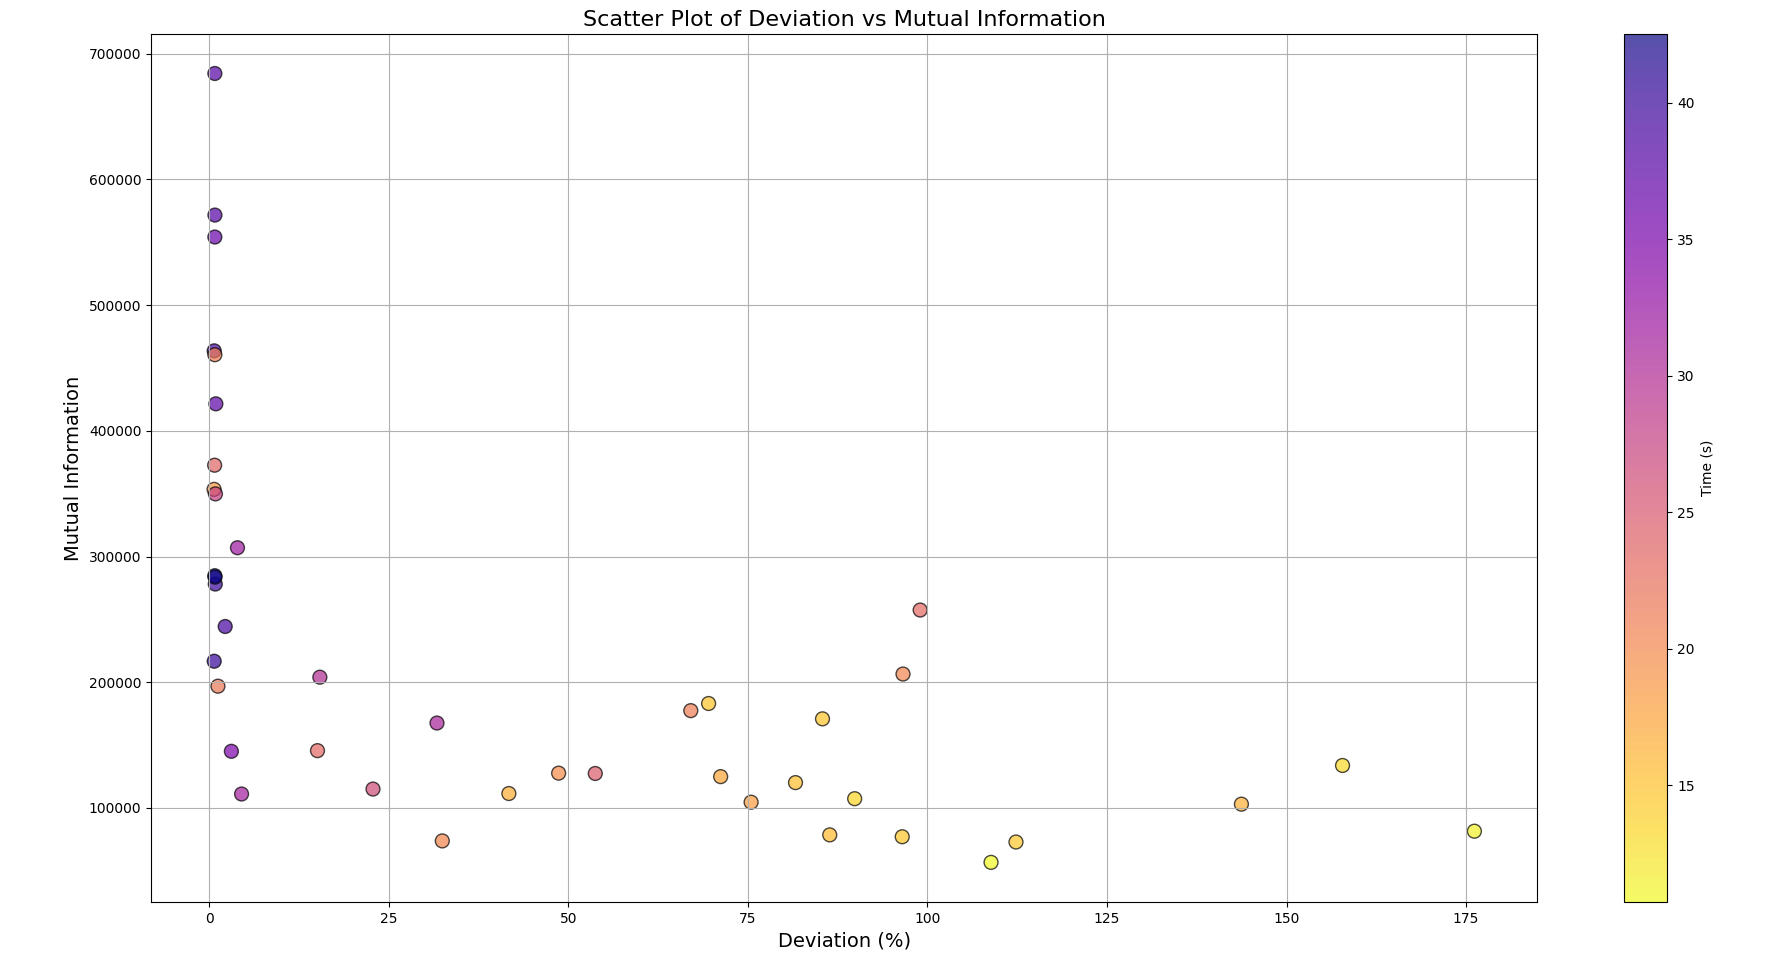
\includegraphics[width=0.7\textwidth]{Chapter 5/RESULTPLOTS/mutual/accmutual.png}
    \caption{Accuracy vs Mutual Information}
    \label{fig:Accuracy_Mutual}
\end{figure}



\subsubsection{Conclusions}

This study demonstrates that UAV navigational accuracy is maintained with mutual information levels up to approximately 20\% of the original image size. Above this threshold, additional mutual information yields diminishing returns in accuracy, indicating an inelastic performance region.
Runtime performance improves proportionally with reduced mutual information, presenting a trade-off between accuracy and computational efficiency. For instance, cropping the image resolution to 1100x635, subtending 300,000 mutual pixels achieves a 1.8-fold runtime reduction with only a 0.1\% increase in error.
These findings emphasize the importance of calibrating resolution levels to balance navigational accuracy and real-time performance. Further, when applying this method, cropping the image towards an aspect ratio of one is recommended to maintain stability as the UAV rotates. Future work should explore adaptive methods that start with reduced mutual information and increase it only when necessary, such as when the UAV is turning around to find its path. 


\subsection{Low-Light Testing}

UAV navigation performance can be significantly impacted by low-light conditions, where keypoint detection and matching accuracy decline due to reduced visibility and increased noise. This study evaluates the robustness of the navigation method under simulated evening and nighttime conditions across five datasets: CITY1, CITY2, ROCKY, DESERT, and AMAZON. Conditions are simulated through adaptions in image brightness, contrast, tint, and noise levels to mimic real-world low-light environments. Evening conditions involve moderate applications of these adjustments, while nighttime conditions feature severe reductions in visibility and increased noise levels. 

The objectives of this study are twofold: firstly, to assess the robustness of the UAV navigation system under low-light conditions by evaluating how evening and nighttime lighting affect the accuracy of navigational estimates; and secondly, to compare the system's performance across diverse environments with varying feature densities under these low-light scenarios.

Representative examples from the CITY1 dataset illustrate these conditions:

\begin{figure}[H]
    \centering
    \begin{minipage}{0.32\textwidth} % Adjust width as necessary
        \centering
        \includegraphics[width=\textwidth]{Chapter 5/RESULTPLOTS/lighting/dayCPT.png}
        \caption{Daytime Image of Cape Town}
        \label{fig:Day_CPT}
    \end{minipage}\hfill
    \begin{minipage}{0.32\textwidth} % Adjust width as necessary
        \centering
        \includegraphics[width=\textwidth]{Chapter 5/RESULTPLOTS/lighting/eveningCPT.png}
        \caption{Evening Image of Cape Town}
        \label{fig:Evening_CPT}
    \end{minipage}\hfill
    \begin{minipage}{0.32\textwidth} % Adjust width as necessary
        \centering
        \includegraphics[width=\textwidth]{Chapter 5/RESULTPLOTS/lighting/nightCPT.png}
        \caption{Night Image of Cape Town}
        \label{fig:Night_CPT}
    \end{minipage}
    
    \caption{Lighting Conditions in Cape Town}
    \label{fig:Lighting_CPT}
\end{figure}


\subsubsection{Results}

Figure \ref{fig:night_evening_rmse} summarizes the accuracy of the navigation method under evening and nighttime conditions for each dataset. Nighttime performance shows that the CITY and ROCKY datasets maintain relatively low RMSE values, indicating resilience to severe low-light environments, while the DESERT and AMAZON datasets exhibit substantial increases in RMSE due to sparse and repetitive features hindering effective keypoint matching. Evening conditions result in minimal degradation of navigational accuracy for most datasets, with the DESERT dataset experiencing a moderate error increase from its initial RMSE of 31.44 m to 156.34 m, corresponding to a 17.51\% RMSE error, which remains usable. 

The performance disparity between datasets underscores the importance of feature density in low-light navigation, with environments rich in distinct landmarks (e.g., CITY and ROCKY) demonstrating greater robustness compared to feature-poor environments (e.g., DESERT and AMAZON).

Overall, the navigation method demonstrates profound resilience in well-featured environments under low-light conditions. However, challenges still remain in feature-sparse environments during nighttime. The usage of additional sensors, such as infrared cameras, could enhance navigational accuracy in these challenging scenarios. 




    \begin{figure}[H]
        \centering
        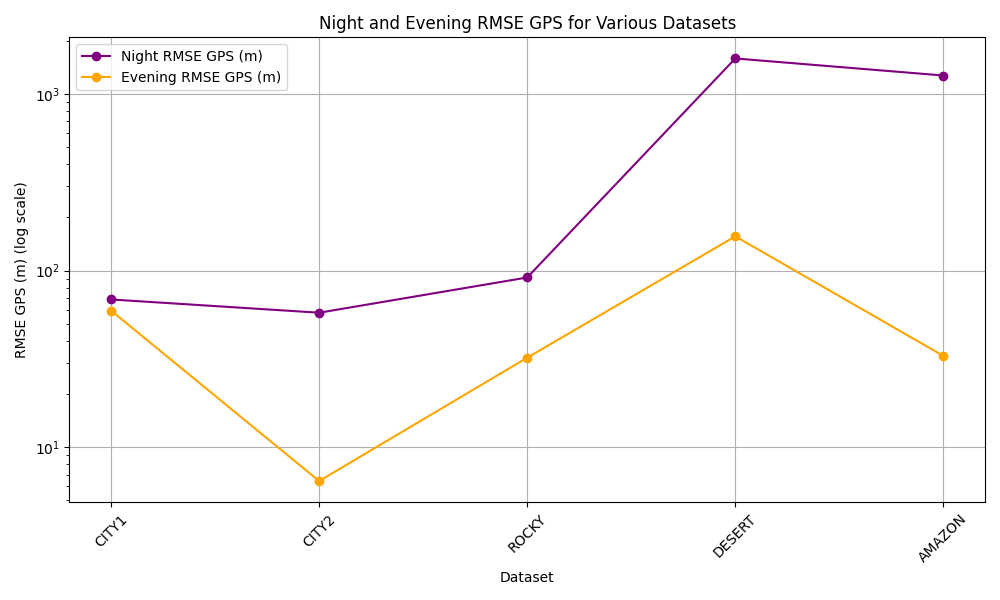
\includegraphics[width=0.7\textwidth]{./Chapter 5/RESULTPLOTS/night_evening_rmse.png}
        \caption{Night and Evening RMSE GPS for Various Datasets}
        \label{fig:night_evening_rmse}
    \end{figure}

    

\section{Results Conclusion}

The results presented in this chapter confirm that the system meets the accuracy and time requirements established in the objectives. The system demonstrated reliable performance across various datasets, including sparse-feature environments, showcasing its ability to generalize effectively. Despite practical limitations such as resolution constraints, performance limitations, and fluctuating terrain feature densities, the system maintained robust accuracy.

The analysis further indicates that accuracy would be significantly improved with access to accurate ground truth headings and known camera parameters, reducing potential sources of error. Furthermore, the system showed resilience under challenging conditions, including low-light scenarios and images with reduced mutual information. Even with limited pixel overlap, the system continued to deliver reliable navigation data.

Overall, the system has proven to be a versatile and effective solution for UAV navigation, capable of sustaining performance under a wide range of operational challenges and environmental conditions.

